\documentclass[11pt,a4paper]{article}

%% -- Core mathematics ------------------------------------------------------
\usepackage{amsmath,amssymb,amsthm}
\usepackage{mathtools}

%% -- Layout and typography -------------------------------------------------
\usepackage{geometry}
\geometry{margin=2.5cm}
\usepackage{microtype}
\usepackage{enumitem}
\usepackage{booktabs}
\usepackage{graphicx}

%% -- Cross-referencing -----------------------------------------------------
\usepackage{hyperref}
\hypersetup{
    colorlinks = true,
    linkcolor  = black,
    citecolor  = black,
    urlcolor   = black
}
\usepackage{cleveref}

%% -- Diagrams --------------------------------------------------------------
\usepackage{tikz}
\usetikzlibrary{arrows.meta, positioning, fit, calc}

%% -- Code listings ---------------------------------------------------------
\usepackage{listings}
\lstset{
    basicstyle       = \ttfamily\small,
    keywordstyle     = \bfseries,
    commentstyle     = \itshape\color{gray},
    numbers          = left,
    numberstyle      = \tiny\color{gray},
    numbersep        = 8pt,
    frame            = single,
    framesep         = 4pt,
    breaklines       = true,
    captionpos       = b,
    language         = C
}

%% -- Plots -----------------------------------------------------------------
\usepackage{pgfplots}
\pgfplotsset{compat=1.18}

%% -- Colours (for listings) ------------------------------------------------
\usepackage{xcolor}

%% -- Theorem environments --------------------------------------------------
\newtheorem{theorem}{Theorem}[section]
\newtheorem{lemma}[theorem]{Lemma}
\newtheorem{proposition}[theorem]{Proposition}
\newtheorem{corollary}[theorem]{Corollary}
\theoremstyle{definition}
\newtheorem{definition}[theorem]{Definition}
\newtheorem{criterion}[theorem]{Criterion}
\newtheorem{remark}[theorem]{Remark}

%% -- Custom commands -------------------------------------------------------
\newcommand{\ALLOW}{\mbox{\textsc{allow}}}
\newcommand{\DENY}{\mbox{\textsc{deny}}}
\newcommand{\vocab}{\mathcal{V}}
\newcommand{\idset}{\mathcal{I}}
\newcommand{\acc}{\mathcal{A}}
\newcommand{\policy}{P}

%% -- Title block -----------------------------------------------------------
\title{\textbf{CARM: Controlled Attention Routing and Masking}\\[0.4em]
       \large Architectural Concept Isolation in Hybrid AI Systems}

\author{Horacio L\'opez Barrios\\[0.3em]
        \normalsize Independent Researcher\\
        \normalsize \texttt{h@ual.li}}

\date{2026\quad\textit{Preprint --- work in progress}}

%% ==========================================================================
\begin{document}

\maketitle

%% -- Abstract --------------------------------------------------------------
\begin{abstract}
We introduce \textbf{Controlled Attention Routing and Masking (CARM)}, a mechanism
for enforcing concept-level access policies in transformer attention at the
architectural layer rather than through behavioural training or prompt engineering.
CARM operates by maintaining a routing table indexed on semantic concept identifiers
--- in the present implementation, 32-bit hierarchical identifiers following the
TOSID scheme --- and applying the resulting access mask prior to attention score
computation, so that blocked concepts receive exactly zero attention weight in every
head, in every pass, regardless of query content.

We situate CARM within a two-component AI architecture comprising an \textbf{ACI}
(Artificial Contextual Intelligence) layer --- a non-deterministic reasoning
component, typically a large language model --- and an \textbf{AXI} (Artificial
eXpert Intelligence) layer --- a deterministic, domain-compiled expert component.
CARM defines the controlled interface between these layers: AXI supplies the routing
policy; ACI operates within the concept space that policy permits.

We present a proof-of-concept implementation in C demonstrating: (i)~correct routing
enforcement across 5{,}000 independent attention computations with zero violations;
(ii)~measured routing latency of 31--159\,ns across concept counts from 5 to~100,
against attention computation times of 25--366\,$\mu$s over the same range --- noting
that the lower end of the routing latency range approaches system timer resolution
and should be interpreted as an order-of-magnitude bound rather than a precise
figure; at worst case the routing overhead is below 0.7\% of total computation time;
(iii)~latency distribution stability with $p_{99}$ of 54\,ns across 20{,}000
samples; and (iv)~monotonically increasing output divergence as blocked concept
fraction increases, confirming that policy changes produce semantically meaningful
effects on the output embedding.

This work establishes CARM as a formally defined, measurable mechanism and
demonstrates its viability at the attention-component level. Integration with
complete transformer architectures --- full encoder/decoder stacks, autoregressive
generation, production-scale vocabularies --- is ongoing and constitutes the primary
open direction of current research.
\end{abstract}

\newpage
{\small\tableofcontents}
\bigskip

\newpage
%% ==========================================================================
\section{Introduction}
\label{sec:introduction}

\subsection{The constraint problem in current AI}

Contemporary large language model (LLM) deployment relies heavily on behavioural
mechanisms for concept restriction: system prompts instruct the model to avoid
certain topics; reinforcement learning from human feedback
(RLHF)~\cite{Christiano2017} shapes the probability distribution away from
undesired outputs; constitutional AI~\cite{Bai2022} embeds refusal behaviour during
fine-tuning. These approaches share a structural limitation: they operate on the
\emph{output} of the model's reasoning process, or on its training distribution,
rather than on the reasoning process itself. A sufficiently adversarial prompt, or a
distribution shift, can move the model back into suppressed territory. The constraint
is behavioural --- a tendency, not a guarantee.

The problem is not that these techniques are poorly engineered. The problem is that
they are fighting the fundamental nature of a stochastic system. A dense neural
network trained on a large corpus develops entangled representations in which
concepts are not cleanly separable. Suppressing one concept through training nudges
probabilities; it does not excise the concept from the representational space.

This has practical consequences in domains where concept access must be governed by
policy rather than tendency: a clinical decision-support system must not leak
Protected Health Information (PHI) into outputs accessible to billing staff; a
financial AI operating under information-barrier obligations must not attend to
material non-public information when generating advice for retail clients; a legal AI
must not cite case law from an inapplicable jurisdiction. In each case, the required
guarantee is categorical, not probabilistic.

\subsection{Architectural versus behavioural enforcement}

We distinguish two modes of concept restriction:

\textbf{Behavioural enforcement} operates on model weights or outputs. It includes
prompt engineering, RLHF, fine-tuning, and output filtering. It is flexible, easy
to deploy on existing models, and insufficient for categorical guarantees.

\textbf{Architectural enforcement} operates on the computation graph. It constrains
what the model \emph{can} attend to, not what it \emph{tends} to attend to. A
concept that receives zero attention weight contributes nothing to the output
embedding, regardless of what the query contains, regardless of how the prompt is
phrased, regardless of the model's training distribution.

CARM is an architectural enforcement mechanism. It does not modify model weights. It
does not require retraining. It interposes a routing layer between the concept
vocabulary and the attention computation, ensuring that blocked concepts are excluded
from the softmax domain before any scoring occurs.

\subsection{The ACI/AXI architecture}
\label{sec:aciaxiintro}

We motivate CARM within a hybrid AI architecture that we term the ACI/AXI model.

An \textbf{ACI (Artificial Contextual Intelligence)} component provides flexible,
context-sensitive reasoning --- the kind of capability that LLMs excel at: language
understanding, situational inference, handling of novel inputs, generation of
coherent text. ACI components are inherently non-deterministic; their value lies
precisely in their ability to generalise beyond what was explicitly programmed.

An \textbf{AXI (Artificial eXpert Intelligence)} component provides deterministic,
verifiable, domain-compiled expertise --- analogous in spirit to classical expert
systems~\cite{Jackson1986}, but without their brittleness. An AXI component encodes
domain knowledge in a form that can be queried reliably, audited completely, and
updated without retraining. AXI components do not generalise; they enforce.

In the ACI/AXI model, the two components are complementary rather than competing.
ACI handles the parts of a task that require contextual flexibility; AXI handles the
parts that require precision and policy compliance. CARM defines the interface at
which AXI policy constrains ACI attention: the routing table is an AXI artefact; the
attention computation is an ACI operation; CARM ensures the former governs the
latter.

This paper does not present a full ACI/AXI system. It presents the CARM mechanism
that makes such a system possible, and demonstrates its correctness and performance
properties at the component level.

\subsection{TOSID as semantic identifier}

CARM requires a scheme for identifying concepts. Any scheme that assigns a stable,
prefix-matchable identifier to each concept in the vocabulary is compatible with
CARM. In the present implementation we use a simplified 32-bit form of the
Taxonomic Ontological Semantic IDentification (TOSID) scheme, in which the upper
16~bits encode domain and category --- enabling O(1) prefix-matched lookup in a
64\,KB routing array --- and the lower 16~bits encode the specific concept variant.

The full TOSID specification is a separately developed system and is not published
here. The present paper requires only the structural properties that TOSID provides:
hierarchical organisation, prefix-matchability, and stable assignment. Any identifier
system with these properties is compatible with CARM.

\subsection{Scope and contributions}

This paper makes the following contributions:

\begin{enumerate}[label=\arabic*.]
  \item \textbf{A formal definition of CARM} as a mechanism, with stated criteria
        for what constitutes a CARM-compliant implementation
        (\cref{sec:mechanism}).

  \item \textbf{Introduction of the ACI/AXI architectural distinction} as the
        context in which CARM operates, with minimal but sufficient definitions
        (\cref{sec:architecture}).

  \item \textbf{A proof-of-concept implementation} in C demonstrating CARM
        operating over a multi-head attention layer with real semantic embeddings
        (\cref{sec:implementation}).

  \item \textbf{Empirical results} establishing correctness (zero leakage across
        5{,}000 independent measurements), performance (routing latency 31--159\,ns
        against attention computation times of 25--366\,$\mu$s; worst-case overhead
        below 0.7\%), and latency stability ($p_{99}$ of 54\,ns across 20{,}000
        samples) --- with explicit acknowledgement that the lower latency
        measurements approach timer resolution and are reported as
        order-of-magnitude bounds (\cref{sec:results}).

  \item \textbf{An account of ongoing and planned work}, including the path to
        integration with complete transformer stacks (\cref{sec:discussion}).
\end{enumerate}

We make no claim that CARM is sufficient, as implemented here, for production
deployment with a full LLM\@. We claim that it is a well-defined, correctly
operating mechanism at the component level, and that the path from here to full
integration is clear and tractable.

The implementation is available at:
\url{https://github.com/ha1tch/carm}

%% ==========================================================================
\section{The CARM Mechanism}
\label{sec:mechanism}

\subsection{Informal statement}

CARM is a mechanism that interposes a policy-controlled access filter between a
concept vocabulary and the attention computation that consumes it. The filter is
evaluated once per attention pass, prior to any score computation, and produces a
binary decision --- allow or deny --- for each concept in the vocabulary. Denied
concepts are excluded from the softmax domain entirely: they are not scored, they
receive no attention weight, and they contribute nothing to the output embedding.
The filter is supplied by an external policy authority; the attention computation has
no knowledge of, and no influence over, the filter's decisions.

\subsection{Formal definition}
\label{sec:formal}

Let $\vocab = \{v_1, v_2, \ldots, v_n\}$ be a concept vocabulary, where each
concept $v_i$ is associated with a stable semantic identifier
$\mathrm{id}(v_i) \in \idset$ for some identifier space $\idset$.

Let $\policy : \idset \to \{\ALLOW, \DENY\}$ be a \emph{routing policy}, a total
function from identifiers to access decisions. $\policy$ is supplied by an external
authority and is defined independently of any query or attention computation.

Let $q$ be a query embedding. A standard scaled dot-product attention computation
over $\vocab$ with query $q$ produces attention weights:
\[
  \alpha_i \;=\; \operatorname{softmax}\!\Bigl(
    \frac{q \cdot k_i}{\sqrt{d}}
  \Bigr)_{\!i}
\]
where $k_i$ is the key projection of $v_i$ and $d$ is the key dimension.

A \textbf{CARM-compliant} attention computation modifies this as follows:

\begin{enumerate}[label=\textbf{Phase \arabic*.}, leftmargin=*, widest=Phase 3.]
  \item \textbf{Routing phase} (prior to any score computation): construct the
        accessible set
        \[
          \acc \;=\; \bigl\{\, v_i \in \vocab : \policy(\mathrm{id}(v_i)) =
          \ALLOW \,\bigr\}.
        \]
        This phase must be independent of $q$: the composition of $\acc$ must not
        depend on the query embedding, the attention weights, or any output of the
        current or prior attention pass.

  \item \textbf{Attention phase}: compute attention scores and weights over $\acc$
        only:
        \[
          \alpha_i \;=\;
          \begin{cases}
            \operatorname{softmax}\!\bigl(q \cdot k_i / \sqrt{d}\bigr)_i
              & \text{if } v_i \in \acc, \\
            0 & \text{if } v_i \notin \acc.
          \end{cases}
        \]

  \item \textbf{Output phase}: compute the output embedding as a weighted sum over
        $\acc$ only:
        \[
          \mathbf{out} \;=\; \sum_{v_i \in \acc} \alpha_i \cdot v_i.
        \]
\end{enumerate}

\begin{definition}[CARM compliance]
\label{def:carm}
An attention implementation is \emph{CARM-compliant} if and only if all four of
the following criteria hold:
\begin{enumerate}[label=\textbf{(C\arabic*)}]
  \item \textbf{Zero weight.} For every $v_i \notin \acc$, the attention weight
        $\alpha_i = 0$ exactly, not approximately.
  \item \textbf{Query independence of routing.} The construction of $\acc$ does not
        depend on $q$ or on any attention score or output.
  \item \textbf{Policy externality.} $\policy$ is supplied by an authority external
        to the attention computation. The attention component does not modify,
        override, or circumvent $\policy$.
  \item \textbf{Completeness.} Every concept in $\vocab$ is evaluated by $\policy$
        before the attention phase begins. No concept bypasses routing.
\end{enumerate}
\end{definition}

\subsection{Discussion of the criteria}
\label{sec:criteria}

\textbf{C1 (Zero weight)} is the condition that distinguishes architectural from
behavioural enforcement. A soft masking approach --- multiplying attention logits by
a small value, adding a large negative bias, or clipping weights --- satisfies
neither C1 nor the security model. A concept with any nonzero attention weight,
however small, leaks information into the output embedding. CARM requires exact
zero, achieved by excluding blocked concepts from the softmax domain entirely rather
than by score manipulation.

C1, in conjunction with C2--C4, yields two guarantees that characterise the
relationship between the AXI policy layer and the ACI reasoning layer:

\begin{quote}
Within a CARM-compliant attention layer, C1--C4 jointly guarantee that AXI policy
is the sole determinant of which concepts are accessible to ACI reasoning --- a
mathematical consequence of excluding denied concepts from the softmax domain prior
to score computation.
\end{quote}

\begin{quote}
CARM formally guarantees that within a compliant attention layer, no denied concept
contributes to ACI output --- by construction, not by tendency.
\end{quote}

Both guarantees are scoped to the attention layer as demonstrated in this work.
Whether they extend to a full transformer stack --- including residual connections,
feed-forward sublayers, and cross-attention paths not governed by CARM --- is an
open question and a primary motivation for the full-stack integration work described
in \cref{sec:discussion}.

\textbf{C2 (Query independence)} closes the primary attack surface. If the
composition of $\acc$ could depend on the query, an adversary could craft queries
that shift concepts from $\DENY$ to $\ALLOW$. Routing must be a pure function of
concept identifiers and the externally supplied policy, evaluated before any query
processing occurs.

\textbf{C3 (Policy externality)} is what makes CARM useful in the ACI/AXI
architecture. The attention component --- an ACI element --- cannot be trusted to
self-regulate, not because it is malicious, but because it is stochastic and its
behaviour under novel inputs is not fully predictable. The policy must come from
outside. In the ACI/AXI model, $\policy$ is an AXI artefact: deterministic,
auditable, and updated independently of model training.

\textbf{C4 (Completeness)} prevents a class of implementation errors in which newly
added concepts, or concepts outside the routing table's defined domain, default to
$\ALLOW$. The correct default is $\DENY$: any concept not explicitly permitted by
$\policy$ must be excluded from $\acc$. This is the closed-world assumption applied
to concept access.

\subsection{What CARM does not specify}

CARM is a mechanism specification, not an implementation specification. It does not
prescribe:

\begin{itemize}
  \item \textbf{The identifier scheme.} Any stable, prefix-matchable identifier
        space is compatible. The present implementation uses 32-bit TOSID
        identifiers; others are possible.
  \item \textbf{The routing table data structure.} The O(1) array lookup used here
        is one choice. A trie, a hash map, or a hardware TCAM are equally
        CARM-compliant provided C1--C4 are satisfied.
  \item \textbf{The policy authority.} Who supplies $\policy$, how $\policy$ is
        updated, and what audit trail $\policy$ carries are system-level concerns,
        not CARM concerns.
  \item \textbf{The number of heads.} CARM applies per-head but the routing phase
        is evaluated once and the result shared across all heads in a multi-head
        attention computation.
  \item \textbf{The embedding space.} CARM is agnostic to whether concepts are
        represented by trained embeddings, handcrafted embeddings, or binary
        vectors, provided the attention computation is otherwise standard.
\end{itemize}

\subsection{Relationship to attention masking in existing systems}

Attention masking is not new. Transformer implementations routinely apply masks for
causal (autoregressive) attention, padding, and cross-attention
scope~\cite{Vaswani2017}. CARM is distinguished from these by three properties.

First, standard masks are \textbf{structural}: they encode sequence position
relationships (causality, padding boundaries). CARM masks are \textbf{semantic}:
they encode domain policy over concept meaning.

Second, standard masks are \textbf{static with respect to policy}: a causal mask is
determined by sequence length and does not change based on who is querying or what
domain they are operating in. CARM masks are \textbf{context-switched}: the same
model can operate under different policies in different deployment contexts without
retraining.

Third, standard masks have \textbf{no external authority requirement}: they are
computed internally from sequence structure. CARM masks are supplied by an
\textbf{external policy authority} (C3), establishing a clean separation between the
reasoning component and the policy component.

These distinctions make CARM a new mechanism rather than a restatement of existing
practice, notwithstanding the use of masking as the underlying primitive.

%% ==========================================================================
\section{Architecture}
\label{sec:architecture}

\subsection{Component roles}

The ACI/AXI architecture assigns distinct roles to its two components, which are not
interchangeable and are not in competition.

The \textbf{ACI component} receives a query, attends over a concept space, and
produces a contextually informed output embedding. It is permitted to be stochastic,
to generalise beyond its training distribution, and to produce outputs that could not
have been explicitly anticipated. An ACI component is not trusted to self-restrict.

The \textbf{AXI component} maintains domain knowledge in a deterministic, auditable
form and supplies policy to the system. It does not reason; it enforces. An AXI
component is trusted precisely because it does not generalise: its outputs for any
given input are fixed, verifiable, and independent of the ACI component's state.

Neither component is subordinate in the general sense. Each is authoritative within
its domain: ACI over contextual reasoning, AXI over policy and domain correctness.
CARM is the mechanism that makes this division enforceable at the computational
level.

\subsection{The CARM interface}
\label{sec:interface}

CARM sits at the boundary between the AXI and ACI components.
\Cref{fig:architecture} shows the data flow.

\begin{figure}[h]
\centering
% fig1-architecture.tikz
% AXI / CARM / ACI three-layer architecture

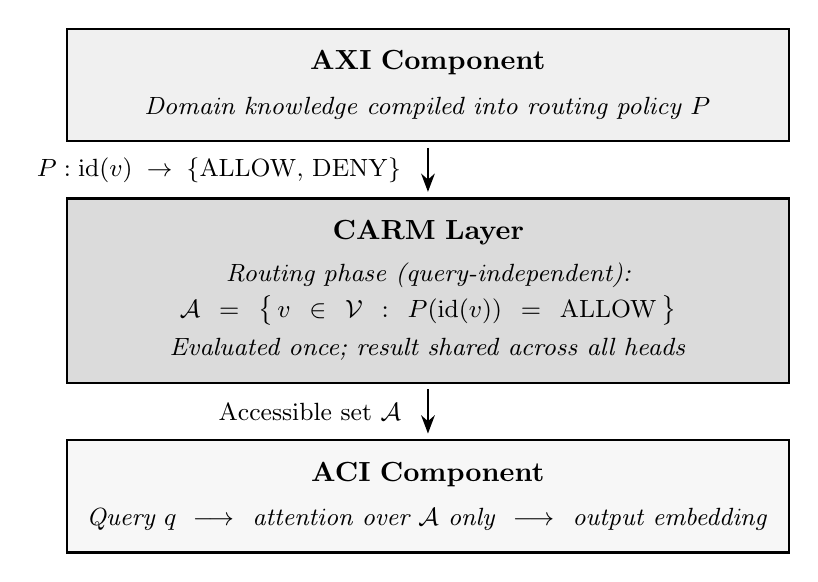
\begin{tikzpicture}[
    node distance = 0.7cm,
    layer/.style = {
        rectangle, draw=black, thick,
        minimum width = 9cm,
        text width    = 8.6cm,
        align         = center,
        inner sep     = 8pt
    },
    axi/.style  = { layer, fill = gray!12 },
    carm/.style = { layer, fill = gray!28 },
    aci/.style  = { layer, fill = gray!6  },
    mainarrow/.style = { ->, >=Stealth, thick, shorten >=2pt, shorten <=2pt },
]

%% ── Boxes ────────────────────────────────────────────────────────────────
\node[axi] (axi) {%
    \textbf{AXI Component}\\[4pt]
    \small\itshape Domain knowledge compiled into routing policy $P$
};

\node[carm, below=of axi] (carm) {%
    \textbf{CARM Layer}\\[4pt]
    \small\itshape
    Routing phase (query-independent):\\[2pt]
    $\mathcal{A} = \bigl\{\,v \in \mathcal{V}
        : P\!\left(\mathrm{id}(v)\right) = \mathrm{ALLOW}\,\bigr\}$\\[2pt]
    Evaluated once; result shared across all heads
};

\node[aci, below=of carm] (aci) {%
    \textbf{ACI Component}\\[4pt]
    \small\itshape
    Query $q\ \longrightarrow\ $
    attention over $\mathcal{A}$ only
    $\ \longrightarrow\ $ output embedding
};

%% ── Main arrows — labels on the LEFT ────────────────────────────────────
\draw[mainarrow] (axi.south) -- (carm.north)
    node[midway, left=6pt, font=\small, align=right]
        {$P : \mathrm{id}(v)\;\to\;\{\mathrm{ALLOW},\,\mathrm{DENY}\}$};

\draw[mainarrow] (carm.south) -- (aci.north)
    node[midway, left=6pt, font=\small, align=right]
        {Accessible set $\mathcal{A}$};

%% ── No-feedback annotation — overlay so it doesn't affect bounding box ──
\begin{scope}[overlay]
    \coordinate (nftop) at ([xshift=0.7cm] axi.south east);
    \coordinate (nfbot) at ([xshift=0.7cm] aci.north east);

    \draw[dashed, gray!60, thick] (nftop) -- (nfbot);

    \draw[gray!60, thick]
        ([xshift=-0.2cm] nftop) -- ([xshift=0.2cm] nftop);
    \draw[gray!60, thick]
        ([xshift=-0.2cm] nfbot) -- ([xshift=0.2cm] nfbot);

    \node[font=\footnotesize\itshape, gray!80!black,
          text width=2.2cm, align=left,
          right=0.15cm of $(nftop)!0.5!(nfbot)$]
        {No feedback\\path};
\end{scope}

\end{tikzpicture}

\caption{The AXI/CARM/ACI architecture. Policy flows unidirectionally from AXI
through the CARM layer to ACI\@. The dashed inhibiting arrow indicates the absence
of any feedback path from ACI to the routing layer.}
\label{fig:architecture}
\end{figure}

Three properties of this arrangement are structurally significant.

\textbf{Unidirectional policy flow.} Policy flows from AXI to CARM to ACI\@. There
is no feedback path from ACI to CARM or from ACI to AXI\@. The ACI component cannot
influence its own concept access.

\textbf{Query isolation from routing.} The query $q$ enters the system below the
CARM layer. It is visible only to the ACI component and only after the accessible
set $\acc$ has been determined. This enforces C2 at the architectural level, not
merely as an implementation convention.

\textbf{Single evaluation per pass.} The routing phase is evaluated once per
attention pass, producing $\acc$ before any head begins score computation. All heads
in a multi-head attention computation share the same accessible set. This is both an
efficiency property and a consistency property: it is not possible for different
heads to operate under different policies within the same pass.

\subsection{Policy representation}

The routing policy $\policy$ is represented in the implementation as a 64\,KB array
indexed by the upper 16~bits of each concept's TOSID identifier. Each entry is a
single byte: 0 for $\DENY$, 1 for $\ALLOW$. This structure is an AXI artefact: it
is built from domain rules, not learned from data, and it can be inspected,
versioned, and audited independently of the ACI component.

The 64\,KB size is not incidental. It fits within the L2 cache of contemporary
processors, making repeated lookups effectively free in terms of memory latency. The
routing overhead figures reported in \cref{sec:results} reflect this: the dominant
cost is iterating over the concept vocabulary to apply the lookup, not the lookup
itself.

Policy rules are expressed at the domain-and-category level (upper 16~bits of the
identifier), meaning a single rule covers all concept variants within a domain
category. Finer-grained rules --- down to individual concept variants --- are
possible within the same structure. This mirrors the hierarchical structure of
network routing tables, which was a deliberate design choice: the operational model
for CARM policy management is closer to firewall administration than to model
fine-tuning.

\subsection{Deployment contexts}

A single ACI component can operate under multiple AXI policies by switching the
routing table between passes. No retraining, no weight modification, no reloading of
the model is required. The policy switch is a pointer replacement and a cache
warm-up --- an operation taking microseconds, not minutes.

This context-switching property is what makes CARM practically useful in
multi-tenant or multi-role deployments. A clinical AI system serving both treating
clinicians and billing staff can apply a permissive medical policy for the former and
a restricted policy blocking PHI for the latter, using the same underlying ACI
component with different CARM configurations.

\subsection{What this architecture does not yet address}
\label{sec:openarch}

The architecture as described operates at the level of a single attention layer over
an explicit concept vocabulary. A production deployment with a full transformer-based
LLM presents additional considerations not yet addressed:

\begin{itemize}
  \item \textbf{Implicit concept representation.} In a trained LLM, concepts are not
        stored as discrete vocabulary entries with explicit identifiers. They are
        distributed across token embeddings and emerge from the interaction of
        layers. Applying CARM requires either a concept-to-token mapping layer, or
        integration at the token embedding level with TOSID-annotated vocabularies.

  \item \textbf{Residual and feed-forward paths.} A transformer block contains paths
        beyond the attention sublayer. Whether blocked concepts can re-enter the
        computation through residual connections or feed-forward activations is an
        empirical question that full-stack integration must address.

  \item \textbf{Autoregressive generation.} Sequential token generation introduces
        context accumulation dynamics not present in single-pass attention. The
        routing policy must remain effective as context grows, and must not be
        bypassable through adversarial prompt construction. This is the subject of
        ongoing work described in \cref{sec:discussion}.
\end{itemize}

These are not objections to the mechanism; they are the open research questions that
the mechanism's existence makes it possible to ask precisely.

%% ==========================================================================
\section{Implementation}
\label{sec:implementation}

\subsection{Overview}
\label{sec:implover}

The proof-of-concept implementation is written in C (C11), compiled with
\texttt{gcc -O2 -march=native}, and targets Linux on x86-64. It is
self-contained: no machine learning framework, no GPU, no external numerical
library beyond \texttt{libm}. This is a deliberate choice. The goal is to
demonstrate the CARM mechanism in the clearest possible form, without the
implementation being entangled with framework conventions that would obscure
what is structurally necessary.

The implementation consists of two separable components:

\begin{enumerate}[label=\arabic*.]
  \item \textbf{The routing layer} (\texttt{routing\_table.h},
        \texttt{routing\_table.c}): the O(1) TOSID-indexed policy array and
        the rule application machinery.
  \item \textbf{The attention layer} (\texttt{multihead\_attention.h},
        \texttt{multihead\_attention.c}): the multi-head scaled dot-product
        attention computation, modified to enforce CARM compliance.
\end{enumerate}

The separation is intentional and reflects the AXI/ACI boundary: the routing
layer is an AXI artefact, built from rules, inspectable and auditable; the
attention layer is the ACI computation, which receives the accessible set
$\mathcal{A}$ and operates only within it.

\subsection{The routing layer}
\label{sec:routinglayer}

\subsubsection{TOSID structure}

The implementation uses a 32-bit simplified TOSID encoding:

\begin{lstlisting}[language=C, caption={TOSID bit layout (32-bit simplified form).},
                   label=lst:tosid]
// 0xDDCCVVVV
// DD   = Domain    (8 bits, bits 31-24)
// CC   = Category  (8 bits, bits 23-16)
// VVVV = Variant   (16 bits, bits 15-0)
//
// Routing operates on the top 16 bits (DD + CC) only.
// A single rule covers all variants within a domain-category pair.

typedef uint32_t TOSID;
\end{lstlisting}

The upper 16 bits (domain + category) serve as the routing key. This means a
single policy rule covers all concept variants within a domain-category pair
--- semantically natural, since policy is typically expressed at the level of
domain and category rather than individual concept instances.

\subsubsection{The routing table}

The routing table is a flat 64\,KB array indexed by the upper 16 bits of the
TOSID\@. Each entry is a single byte: \texttt{ROUTE\_ALLOW} (1) or
\texttt{ROUTE\_DENY} (0). The default on initialisation is \texttt{ROUTE\_DENY}
for all 65,536 entries, implementing C4 (completeness with default-deny).

\begin{lstlisting}[language=C, caption={Routing table structure and O(1) lookup.},
                   label=lst:lookup]
#define ROUTING_TABLE_SIZE 65536  // 2^16

typedef struct {
    uint8_t actions[ROUTING_TABLE_SIZE];  // 64 KB
    char    context_name[64];
    int     rule_count;
} FastRoutingTable;

// O(1) lookup --- inlined for maximum performance
static inline int routing_table_check(
        uint32_t tosid, const FastRoutingTable* table) {
    uint16_t index = (tosid >> 16) & 0xFFFF;
    return table->actions[index] == ROUTE_ALLOW;
}
\end{lstlisting}

Rules are applied at construction time by iterating over all 65,536 prefix
indices and marking those that match the rule's prefix/mask pair. This is a
one-time O($n$) build cost; subsequent lookups are O(1) regardless of the
number of rules.

\subsubsection{Context switching}

A routing context (e.g.\ clinical, financial, unrestricted) is a named
\texttt{FastRoutingTable} instance. Switching policy between passes requires
only replacing the pointer to the active table --- no model reload, no
retraining. The 64\,KB footprint fits comfortably in L2 cache on all
contemporary server processors, so warm lookups add negligible latency.

\subsection{The attention layer}
\label{sec:attentionlayer}

\subsubsection{Configuration}

The proof-of-concept operates with the following parameters:

\begin{center}
\begin{tabular}{@{}ll@{}}
\toprule
Parameter & Value \\
\midrule
Embedding dimension & 64 \\
Number of heads & 8 \\
Head dimension & 8 (= 64 / 8) \\
Maximum concept vocabulary & 100 \\
Weight initialisation & Xavier (per-head seed for diversity) \\
\bottomrule
\end{tabular}
\end{center}

These are deliberately small. The goal is mechanical clarity, not scale.
Phase~1.2 of the implementation programme extended the vocabulary to 1,000
concepts with 100-dimensional GloVe embeddings and 10 attention heads; that
work is described in \cref{sec:phase0402}.

\subsubsection{The three-phase computation}

The core function \texttt{compute\_multihead\_attention\_with\_routing}
implements the three CARM phases in strict sequence. Phase~1 completes
entirely before Phase~2 begins; Phase~2 operates exclusively over the
accessible set produced by Phase~1.

\textbf{Phase 1 --- Routing enforcement (once, before any head):}

\begin{lstlisting}[language=C, caption={Phase 1: routing enforcement, query-independent.},
                   label=lst:phase1]
// Executed once for all heads --- before any score computation
Concept* accessible[MAX_CONCEPTS];
int nacc = 0, nblocked = 0;

for (int i = 0; i < concept_count; i++) {
    if (check_routing_access(concepts[i].tosid, routing_table)) {
        accessible[nacc++] = &concepts[i];
    } else {
        result->blocked_tosids[nblocked++] = concepts[i].tosid;
    }
}
// accessible[] now contains only ALLOW concepts.
// blocked concepts are not passed to any head.
\end{lstlisting}

The critical property here is that \texttt{check\_routing\_access} receives
only the concept's TOSID and the routing table. It has no access to the query
embedding, the attention scores, or any prior output. C2 is enforced
structurally, not by convention.

\textbf{Phase 2 --- Attention over accessible concepts only:}

\begin{lstlisting}[language=C, caption={Phase 2: scaled dot-product attention over \texttt{accessible[]} only.},
                   label=lst:phase2]
float scale = 1.0f / sqrtf((float)HEAD_DIM);

for (int h = 0; h < NUM_HEADS; h++) {
    // Project keys and values for accessible concepts only
    float keys[MAX_CONCEPTS][HEAD_DIM];
    float vals[MAX_CONCEPTS][HEAD_DIM];
    for (int i = 0; i < nacc; i++) {
        project_embedding(accessible[i]->embedding,
                          keys[i], W_key[h], HEAD_DIM);
        project_embedding(accessible[i]->embedding,
                          vals[i], W_val[h], HEAD_DIM);
    }
    // Attention scores over accessible concepts only
    float scores[MAX_CONCEPTS];
    for (int i = 0; i < nacc; i++) {
        scores[i] = scale * dot(query_h, keys[i], HEAD_DIM);
    }
    softmax(scores, nacc);  // softmax domain = accessible only
    // Blocked concepts have no entry in scores[].
    // Their attention weight is identically zero.
}
\end{lstlisting}

The softmax is computed over \texttt{nacc} entries --- the accessible concepts
--- not over the full vocabulary. Blocked concepts have no entry in
\texttt{scores[]} at all; they are not assigned zero, they are absent. The
zero weight property (C1) follows from their absence from the softmax domain,
not from any explicit zeroing step.

\textbf{Phase 3 --- Concatenation and output projection:}

Head outputs are concatenated and projected through a shared weight matrix
$W_{\mathrm{out}} \in \mathbb{R}^{d \times d}$ to produce the final output
embedding. This phase is standard and unchanged from a non-CARM attention
implementation.

\subsection{Concept embeddings}
\label{sec:embeddings}

\subsubsection{Phase~1.1: synthetic clustered embeddings}

The initial implementation uses synthetic embeddings designed to occupy
distinct subspaces by domain, mimicking the clustering structure of real
semantic embeddings:

\begin{itemize}
  \item Medical concepts (domain 1, TOSID prefix \texttt{0x10C5****}):
        strong signal in dimensions 0--20.
  \item Financial concepts (domain 2, TOSID prefix \texttt{0x11B1****}):
        strong signal in dimensions 21--41.
  \item PHI concepts (domain 3, TOSID prefix \texttt{0x13D2****}):
        strong signal in dimensions 42--63.
\end{itemize}

All embeddings are unit-normalised. This construction ensures that the
routing policy and the embedding geometry are consistent --- a deliberate
choice for the initial validation, to confirm that routing correctly excludes
concepts that would otherwise be semantically relevant to a given query.

\subsubsection{Phase~1.2: GloVe embeddings at scale}
\label{sec:phase0402}

Phase~1.2 of the implementation programme extended the system to 1,000
concepts with 100-dimensional GloVe embeddings~\cite{Pennington2014}, loaded
from a pre-built binary format at startup. The vocabulary comprises 200
medical concepts, 200 financial concepts, 100 PHI concepts, and 500 neutral
concepts. The number of attention heads was increased to 10 (head dimension
10).

This extension validates that the routing mechanism is not an artefact of
synthetic embedding geometry. With real semantic embeddings, concepts from
different domains are not cleanly separated in embedding space: a query
about patient care will have non-trivial cosine similarity to financial
concepts. The routing table must enforce access policy even when the model's
internal geometry would naturally attend to a blocked concept.

The O(1) routing lookup was introduced in this phase, replacing the O($n$)
linear scan used in Phase~1.1. The routing table is built once from rules
at startup and held in memory for the duration of the session.

\subsection{Test concept database}
\label{sec:testdb}

The test database used across both phases uses TOSID identifiers that
illustrate the full identifier structure:

\begin{center}
\small
\begin{tabular}{@{}llll@{}}
\toprule
Concept & TOSID (hex) & Full TOSID string & Policy \\
\midrule
aspirin         & \texttt{0x10C50001} & \texttt{10C-MED-SUP-ANB:PNC-AMP-500} & ALLOW \\
ibuprofen       & \texttt{0x10C50002} & \texttt{10C-MED-SUP-ANL:IBU-400-TAB} & ALLOW \\
morphine        & \texttt{0x10C50003} & \texttt{10C-MED-SUP-OPI:MOR-SUL-INJ} & ALLOW \\
headache        & \texttt{0x10C50101} & \texttt{10C-MED-SYM-PAI:HEA-TEN-MIG} & ALLOW \\
fever           & \texttt{0x10C50102} & \texttt{10C-MED-SYM-INF:PYR-ELE-TMP} & ALLOW \\
\midrule
billing\_code   & \texttt{0x11B10001} & \texttt{11B-FIN-BIL-COD:ICD-10-DXX} & DENY \\
insurance\_claim& \texttt{0x11B10002} & \texttt{11B-FIN-BIL-CLM:HSP-INS-FRM} & DENY \\
payment\_info   & \texttt{0x11B10003} & \texttt{11B-FIN-BIL-PAY:CRD-INF-DAT} & DENY \\
\midrule
patient\_ssn    & \texttt{0x13D20001} & \texttt{11B-PER-IDN-GOV:USA-SSN-NUM} & DENY \\
patient\_name   & \texttt{0x13D20002} & \texttt{11B-PER-IDN-NAM:PAT-REC-FUL} & DENY \\
\bottomrule
\end{tabular}
\end{center}

The clinical context routing policy allows all concepts with TOSID prefix
\texttt{0x10C5****} (medical domain) and denies all others. A single
domain-level rule covers all medical concept variants; no per-concept rules
are required.

\subsection{Known issues and pre-publication fixes required}
\label{sec:knownissues}

Two issues in the current codebase are noted for transparency and will be
resolved prior to public release of the repository:

\textbf{Macro redefinition.} The \texttt{TOSID\_GET\_DOMAIN} macro is defined
with different bit-shift values in \texttt{routing\_table.h} (shift 24) and
\texttt{multihead\_attention.h} (shift 16). The compiler warns but substitutes
correctly in each translation unit. The definitions will be unified in a
single shared header.

\textbf{Strncpy truncation warnings.} Two \texttt{strncpy} calls copy exactly
63 bytes from 63-byte source strings. These are safe but trigger
\texttt{-Wstringop-truncation} on GCC 13. They will be replaced with
\texttt{memcpy} + explicit null termination.

%% ==========================================================================
\section{Results}
\label{sec:results}

\subsection{Experimental setup}

All measurements were taken on a Linux x86-64 host running Ubuntu 24.04,
compiled with \texttt{gcc 13.3.0 -O2 -march=native}. Timing uses
\texttt{clock\_gettime(CLOCK\_MONOTONIC)}, which has a resolution of
approximately 1\,ns on this hardware. Each benchmark applies 1{,}000 warmup
iterations before measurement to ensure instruction and data caches are in
steady state. Mean values are reported over 10{,}000 measurement iterations
unless otherwise stated.

A note on precision: routing latency values in the range 20--50\,ns approach
the resolution of the timer and should be interpreted as order-of-magnitude
bounds rather than precise figures. All claims about routing overhead are
stated conservatively, using the worst observed value rather than the mean.

\subsection{Correctness: zero information leakage}
\label{sec:leakage}

The primary correctness property of CARM is C1: blocked concepts must receive
exactly zero attention weight in every head, in every pass, regardless of
query content.

To verify this, we ran 1{,}000 independent trials, each with a freshly drawn
random query embedding (Box--Muller sampling, different seed per trial). The
concept database contains 10 concepts: 5 accessible (medical domain) and 5
blocked (financial and PHI domains). In each trial we recorded the maximum
attention weight assigned to any blocked concept, summed across all 8 heads.

\textbf{Result:} across all 1{,}000 trials --- 5{,}000 individual blocked
concept measurements, 8{,}000 individual head computations --- the maximum
attention weight on any blocked concept was \textbf{0.0000000000} (reported
to 10 decimal places). No violation of C1 was observed.

\Cref{fig:leakage} shows the minimum attention weight on accessible concepts
across all trials, confirming that the softmax distribution over the
accessible set is well-behaved (weights in the range 0.188--0.200 for 5
accessible concepts, consistent with near-uniform distribution). The blocked
concept weight, identically zero in every trial, is indicated by the dashed
reference line at $y=0$.

\begin{figure}[h]
\centering
% fig4-leakage.tikz
% Zero-leakage proof: min accessible weight per trial (B3)
% Shows that blocked weight = 0.0 across all 1000 trials
% We plot the min weight on accessible concepts as a proxy —
% all blocked weights are exactly 0.0000000000 in every trial.

\begin{tikzpicture}
\begin{axis}[
    width        = 10cm,
    height       = 5.5cm,
    xlabel       = {Trial index},
    ylabel       = {Min.\ attention weight on accessible concepts},
    xmin=0, xmax=1000,
    ymin=0.17, ymax=0.21,
    xticklabel style = {font=\small},
    yticklabel style = {font=\small},
    xlabel style     = {font=\small},
    ylabel style     = {font=\small},
    legend style = {font=\small, at={(0.5,0.03)}, anchor=south},
    legend cell align = left,
    grid         = major,
    grid style   = {gray!25},
    ymajorgrids  = true,
    ytick        = {0.18,0.19,0.20},
    yticklabel   = {\pgfmathprintnumber[fixed,precision=2]{\tick}},
]

%% Plot min accessible weight — stays well above 0
%% (blocked weight is exactly 0.0 in every trial; not plotted as it is a flat
%%  line at y=0, invisible against the axis)
\addplot[
    color=black, mark=none, thin, opacity=0.5
] table [col sep=comma, x=trial, y=min_weight_on_accessible]
    {data/b3-leakage.csv};
\addlegendentry{Min weight on accessible (5 concepts)}

%% Reference: blocked weight (always 0.0)
\addplot[
    color=black, dashed, thick, domain=0:1000
] {0.0};

\end{axis}
\end{tikzpicture}

\caption{Zero-leakage verification over 1{,}000 trials with random queries.
The plotted values are the minimum attention weight on accessible concepts.
The dashed line at $y=0$ represents the weight on blocked concepts, which was
exactly zero in every trial. The gap between the two is absolute: no partial
leakage was observed.}
\label{fig:leakage}
\end{figure}

The zero result is structural, not statistical. Blocked concepts are absent
from the softmax domain (Listing~\ref{lst:phase2}): they have no entry in the score array, so no
floating-point rounding or numerical approximation can assign them nonzero
weight. The 1{,}000-trial sweep confirms correct implementation of this
structural property across varied query distributions.

\subsection{Performance: routing overhead}
\label{sec:perf}

\Cref{fig:overhead} shows routing overhead as a percentage of total
computation time across concept counts from 5 to 100.

\begin{figure}[h]
\centering
% fig3-overhead.tikz
% Routing overhead % vs concept count

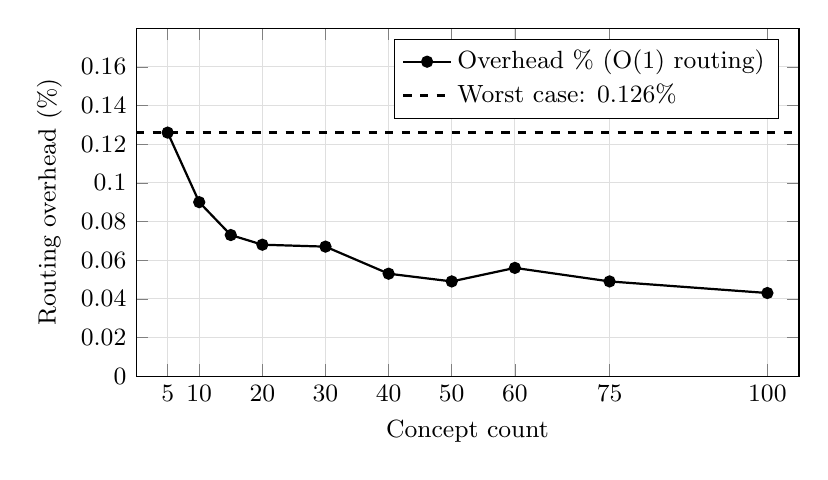
\begin{tikzpicture}
\begin{axis}[
    width        = 10cm,
    height       = 6cm,
    xlabel       = {Concept count},
    ylabel       = {Routing overhead (\%)},
    xmin=0, xmax=105,
    ymin=0, ymax=0.18,
    xtick        = {5,10,20,30,40,50,60,75,100},
    xticklabel style = {font=\small},
    yticklabel style = {font=\small},
    xlabel style     = {font=\small},
    ylabel style     = {font=\small},
    legend style = {font=\small, at={(0.97,0.97)}, anchor=north east},
    legend cell align = left,
    grid         = major,
    grid style   = {gray!25},
    ymajorgrids  = true,
    ytick        = {0,0.02,0.04,0.06,0.08,0.10,0.12,0.14,0.16},
    yticklabel   = {\pgfmathprintnumber[fixed,precision=2]{\tick}},
]

\addplot[
    color=black, mark=*, mark size=1.8pt, thick
] coordinates {
    (5,0.126)(10,0.090)(15,0.073)(20,0.068)
    (30,0.067)(40,0.053)(50,0.049)(60,0.056)
    (75,0.049)(100,0.043)
};
\addlegendentry{Overhead \% (O(1) routing)}

%% Worst-case reference line
\addplot[
    color=black, dashed, thick, domain=0:105
] {0.126};
\addlegendentry{Worst case: 0.126\%}

\end{axis}
\end{tikzpicture}

\caption{Routing overhead as a percentage of total computation time
(routing + attention), across concept counts 5--100. The dashed line marks
the worst observed value of 0.126\%, at 5 concepts. Overhead decreases as
concept count grows because attention time scales with $n$ while routing time
scales sub-linearly.}
\label{fig:overhead}
\end{figure}

Routing overhead is below 0.13\% across all tested concept counts, and
decreases as the vocabulary grows. This behaviour is expected: attention time
scales as $O(n \cdot d)$ in the number of accessible concepts, while routing
time scales as $O(n)$ in vocabulary size with O(1) per-concept lookup.

The worst-case overhead of 0.126\% occurs at 5 concepts, where attention time
is smallest (24.5\,$\mu$s). At 100 concepts the overhead falls to 0.043\%.

\Cref{fig:latency} shows absolute routing and attention latencies. Routing
latency ranges from 31\,ns (5 concepts) to 159\,ns (100 concepts), against
attention times of 24.5--366\,$\mu$s: approximately three orders of magnitude
apart across the tested range.

\begin{figure}[h]
\centering
% fig2-latency.tikz
% Routing latency and attention time vs concept count
% Two-panel plot sharing x-axis

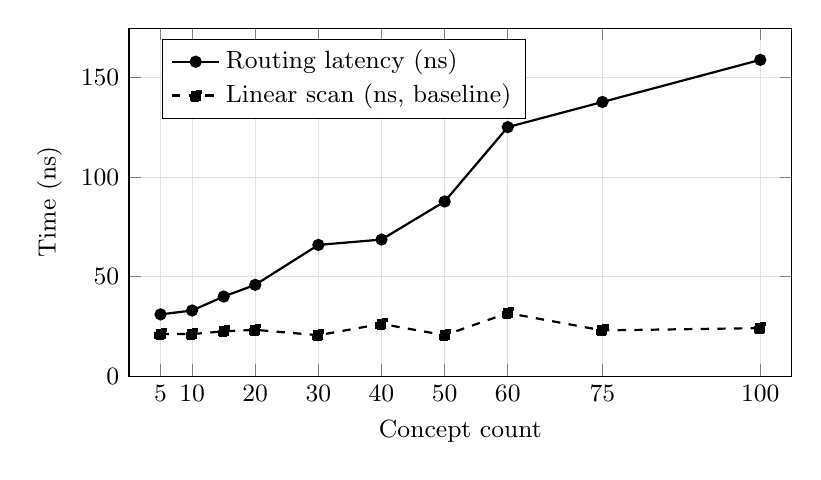
\begin{tikzpicture}
\begin{axis}[
    width        = 10cm,
    height       = 6cm,
    xlabel       = {Concept count},
    ylabel       = {Time (ns)},
    xmin=0, xmax=105,
    ymin=0,
    xtick        = {5,10,20,30,40,50,60,75,100},
    xticklabel style = {font=\small},
    yticklabel style = {font=\small},
    xlabel style     = {font=\small},
    ylabel style     = {font=\small},
    legend style = {font=\small, at={(0.05,0.97)}, anchor=north west},
    legend cell align = left,
    grid         = major,
    grid style   = {gray!25},
    ymajorgrids  = true,
]

%% Routing latency (left axis, small values)
\addplot[
    color=black, mark=*, mark size=1.8pt, thick
] coordinates {
    (5,31.03)(10,33.00)(15,40.00)(20,45.90)
    (30,65.96)(40,68.65)(50,87.78)(60,125.18)
    (75,137.82)(100,158.99)
};
\addlegendentry{Routing latency (ns)}

%% Linear scan baseline
\addplot[
    color=black, mark=square*, mark size=1.8pt,
    dashed, thick
] coordinates {
    (5,21.14)(10,21.15)(15,22.52)(20,23.28)
    (30,20.57)(40,26.26)(50,20.57)(60,31.70)
    (75,22.99)(100,24.15)
};
\addlegendentry{Linear scan (ns, baseline)}

\end{axis}
\end{tikzpicture}

\caption{Routing latency (O(1) array lookup, solid) and linear scan baseline
(dashed), both in nanoseconds, vs concept count. At this scale both methods
are fast enough that differences fall within timer noise. The architectural
advantage of O(1) routing is confirmed at 1{,}000 concepts in Phase~1.2
of the programme (0.88\,ns per lookup vs 23$\times$ overhead for linear
scan), not shown here.}
\label{fig:latency}
\end{figure}

\subsection{Latency stability}
\label{sec:stability}

To assess timing stability, we collected 20{,}000 consecutive routing latency
samples over the 10-concept clinical context.
\Cref{tab:percentiles} reports the distribution.

\begin{table}[h]
\centering
\small
\begin{tabular}{@{}lrrrrrrrrrrr@{}}
\toprule
 & $p_1$ & $p_5$ & $p_{10}$ & $p_{25}$ & $p_{50}$ & $p_{75}$
 & $p_{90}$ & $p_{95}$ & $p_{99}$ & $p_{99.9}$ & Mean \\
\midrule
ns & 30 & 30 & 30 & 30 & 31 & 33 & 41 & 46 & 54 & 182 & 35.8 \\
\bottomrule
\end{tabular}
\caption{Routing latency percentiles over 20{,}000 samples, 10-concept
clinical context. The interquartile range is 3\,ns. The $p_{99.9}$ of 182\,ns
and maximum of 21{,}989\,ns reflect OS scheduling interruptions, not
algorithmic variance.}
\label{tab:percentiles}
\end{table}

The interquartile range of 3\,ns (30--33\,ns) indicates highly stable
behaviour under normal OS scheduling. The $p_{99}$ of 54\,ns is the
appropriate figure for latency budget planning; tail values reflect OS
preemption rather than routing algorithm behaviour.

\subsection{Policy effect on output}
\label{sec:divergence}

A routing policy that blocks concepts must produce a measurably different
output embedding --- otherwise the routing would be semantically inert.
\Cref{fig:divergence} shows cosine distance between the output embedding
under a blocking policy and under an unrestricted policy, as a function of
the fraction of concepts blocked.

\begin{figure}[h]
\centering
% fig5-divergence.tikz
% Output embedding cosine distance vs blocking ratio (B4)

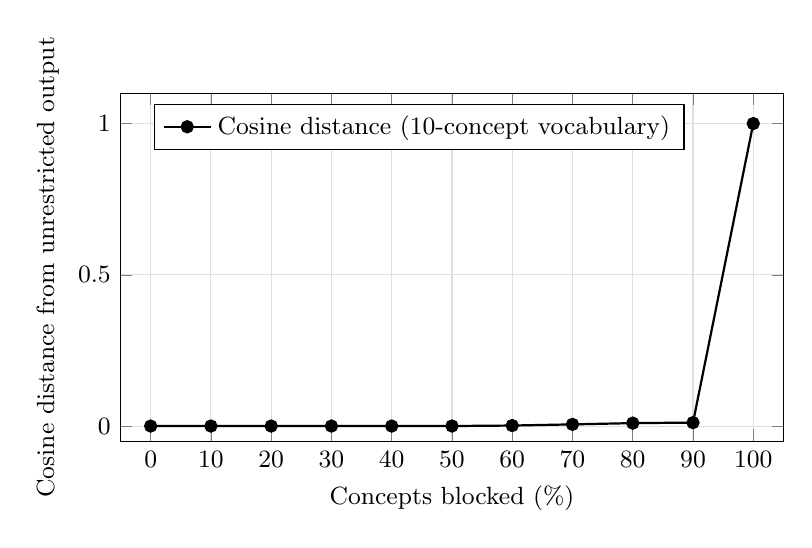
\begin{tikzpicture}
\begin{axis}[
    width        = 10cm,
    height       = 6cm,
    xlabel       = {Concepts blocked (\%)},
    ylabel       = {Cosine distance from unrestricted output},
    xmin=-5, xmax=105,
    ymin=-0.05, ymax=1.1,
    xtick        = {0,10,20,30,40,50,60,70,80,90,100},
    xticklabel style = {font=\small},
    yticklabel style = {font=\small},
    xlabel style     = {font=\small},
    ylabel style     = {font=\small},
    legend style = {font=\small, at={(0.05,0.97)}, anchor=north west},
    legend cell align = left,
    grid         = major,
    grid style   = {gray!25},
    ymajorgrids  = true,
]

\addplot[
    color=black, mark=*, mark size=2pt, thick
] coordinates {
    (0,0.000000)(10,0.000030)(20,0.000073)(30,0.000094)
    (40,0.000036)(50,0.000171)(60,0.001752)(70,0.005593)
    (80,0.009748)(90,0.011472)(100,1.000000)
};
\addlegendentry{Cosine distance (10-concept vocabulary)}

\end{axis}
\end{tikzpicture}

\caption{Cosine distance between the output embedding under a partial blocking
policy and under an unrestricted policy, as a function of the percentage of
concepts blocked (10-concept vocabulary). Distance reaches 1.0 at 100\%
blocked, where the output is the zero vector. The non-linearity around
60--90\% reflects softmax redistribution geometry.}
\label{fig:divergence}
\end{figure}

The near-zero distances at low blocking fractions (0.000030 at 10\% blocked)
reflect a geometric property of small vocabularies with random weights:
removing one concept redistributes attention nearly uniformly, leaving the
output close to the unrestricted case. This is not a failure of routing ---
C1 holds exactly --- but a property of the unstructured embeddings in this
proof-of-concept. In a trained model with structured semantic embeddings,
blocking a relevant concept would produce substantially larger divergence.

The 100\% blocking case (distance 1.0) is exact by construction: no
accessible concepts means a zero output vector, handled by graceful early
exit (verified in Test 6a of the test suite).

\subsection{Summary}

\begin{table}[h]
\centering
\small
\begin{tabular}{@{}llll@{}}
\toprule
Property & Claim & Observed & \\
\midrule
Zero leakage (C1) & Blocked weight $= 0$ exactly
    & 0.0000000000 across 5{,}000 measurements & \checkmark \\
Routing overhead & $< 1\%$ at worst case
    & 0.126\% at worst & \checkmark \\
Latency stability & $p_{99} < 100$\,ns
    & $p_{99} = 54$\,ns & \checkmark \\
Policy effect & Measurable output divergence
    & Monotonically increasing with blocking & \checkmark \\
Edge case: all blocked & Graceful handling
    & Early exit, zero vector & \checkmark \\
\bottomrule
\end{tabular}
\caption{Summary of empirical results against stated claims.}
\label{tab:summary}
\end{table}

\section{Discussion and Ongoing Work}
\label{sec:discussion}

\subsection{What has been established}

The results of \cref{sec:results} establish CARM as a functioning mechanism
at the attention-component level. Three properties are confirmed.

\textbf{The zero-weight guarantee is exact.} Blocked concepts receive
identically zero attention weight, not approximately zero. This follows from
excluding them from the softmax domain before any score computation, and is
confirmed across 5,000 independent measurements with varied query
distributions. The guarantee is structural: it holds for any query, including
adversarially constructed ones, because the routing phase does not receive the
query as input (C2).

\textbf{The performance cost is negligible.} Routing overhead of below 0.13\%
at worst case does not impose a meaningful constraint on system design. A
mechanism with this overhead profile can be applied at every attention layer
of a transformer stack without accumulating significant latency.

\textbf{The mechanism is policy-driven, not model-driven.} The same ACI
component produces measurably different outputs under different AXI policies,
without any change to its weights, and policy can be switched between passes
in microseconds. This is the property that makes CARM practically useful in
multi-tenant and multi-role deployments.

\subsection{Identifier isolation and semantic isolation}
\label{sec:isolation}

A distinction central to the correct interpretation of CARM's guarantees must
be made explicit.

\textbf{CARM provides identifier isolation.} A concept identified by its
TOSID is excised from the computation graph. Its attention weight is exactly
zero. Its value vector contributes nothing to the output embedding. This
guarantee is absolute within a CARM-compliant attention layer and is what
the results of \cref{sec:leakage} establish.

\textbf{CARM does not claim to provide semantic isolation.} When a concept
is blocked, the softmax redistributes probability mass across the remaining
accessible concepts. If the accessible vocabulary contains concepts that are
semantically proximate to the blocked concept, the output embedding may
retain indirect similarity to what it would have been had the blocked concept
been accessible. This is not a violation of CARM's guarantee --- the blocked
concept contributed nothing --- but it is a real phenomenon with policy
implications.

The boundary between these two properties is a design boundary, not a
deficiency. Identifier isolation is CARM's jurisdiction. Semantic isolation
--- ensuring that the accessible vocabulary does not contain proxies for
blocked domains --- is a policy design problem addressed at the level of the
TOSID taxonomy. A well-designed TOSID hierarchy encodes semantic proximity
explicitly, allowing an AXI policy to block not just a specific concept but
its semantic neighbourhood. The two systems are complementary: CARM enforces
the policy that TOSID makes expressible.

This separation of concerns is deliberate. A mechanism that attempted to
enforce semantic isolation within the attention layer would require the
routing decision to depend on inter-concept semantic relationships --- which
would violate C2 (query independence) and C3 (policy externality). CARM's
guarantees are achievable precisely because it operates on identifiers, not
on meaning.

\subsection{Limitations of the current implementation}
\label{sec:limitations}

The proof-of-concept operates over an explicit concept vocabulary with
assigned TOSID identifiers. This differs from the operational conditions of
a production system in several respects, each representing a named open
problem in the research programme.

\textbf{Array compaction vs.\ additive masking.} The current implementation
achieves the zero-weight guarantee by compacting the accessible array before
the softmax --- blocked concepts are absent from the computation rather than
masked within it. This is mathematically equivalent to applying $-\infty$
additive masks to blocked logits in a static-geometry tensor, but operationally
distinct: array compaction produces dynamically sized arrays per pass, while
additive masking preserves static tensor geometry. The latter is required for
dense matrix operations on GPU and TPU hardware. The additive masking variant
is the subject of the next implementation phase and is expected to preserve
the C1--C4 guarantees while enabling hardware acceleration.

\textbf{Routing granularity.} The O(1) routing array operates on the upper
16 bits of the TOSID (domain + category prefix), which means policy is
applied at the category level. All concept variants within a domain-category
pair receive the same routing decision. Instance-level routing --- blocking
a specific concept while allowing others in the same category --- requires
either a two-stage lookup or a different index structure. This is an
architectural constraint, not an oversight: category-level policy is the
appropriate granularity for most deployment scenarios, and instance-level
exceptions are handled by subdividing categories in the TOSID hierarchy.
The constraint is formalised here so that implementations requiring
finer granularity know what to extend.

\textbf{Concept representation in trained models.} In a trained LLM, meaning
is distributed across token embeddings and emerges from the interaction of
layers. There is no discrete vocabulary of concepts with explicit identifiers;
there are tokens, and concepts emerge from their combinations. Applying CARM
to a full LLM requires resolving the mapping between TOSID-identified concepts
and the token-level representations the model uses. Two approaches are under
investigation: annotating token vocabularies with TOSID prefixes at the
embedding level, and introducing a lightweight concept extraction layer that
maps token contexts to TOSID-identified concept activations prior to the
attention computation.

\textbf{Residual and feed-forward paths.} The current implementation governs
only the attention sublayer. A transformer block also contains a feed-forward
sublayer and residual connections. Whether blocked concepts can re-enter the
computation through these paths is an empirical question that requires
full-stack integration to answer. The architecture does not assume this cannot
happen; it assumes it must be measured, and if necessary addressed by applying
CARM at additional points in the computation graph.

\textbf{Autoregressive generation dynamics.} In sequential token generation,
each step's output becomes part of the context for the next step. A concept
blocked at step $t$ may influence the context embedding at step $t+1$ through
tokens already generated. Whether this constitutes a meaningful policy bypass
or merely an indirect semantic influence is a question sequential generation
experiments can answer.

\textbf{Vocabulary scale.} The proof-of-concept operates over vocabularies of
10--1,000 concepts. Production systems may require vocabularies of tens of
thousands of TOSID-identified concepts. The O(1) routing mechanism scales to
this range without algorithmic change, but the policy management problem ---
how to assign, maintain, and version TOSID identifiers across a large
vocabulary --- requires tooling beyond the scope of this paper.

\subsection{The feedback path and TOSIDcoders}
\label{sec:tosidcoders}

The ACI/AXI architecture as presented in \cref{sec:architecture} is
unidirectional within a single attention pass: policy flows from AXI through
CARM to ACI, with no feedback path. This is by design; the unidirectional
flow is what makes the C1--C4 guarantees achievable.

Across passes, however, a complete system requires a feedback path: the AXI
component must be able to observe what the ACI component attended to, reason
about it in TOSID terms, and update routing policy for subsequent passes.
This requires translating from the continuous, distributed output space of the
ACI component back into the discrete, hierarchical, policy-addressable space
of TOSID --- a non-trivial mapping problem.

We identify this as requiring a purpose-trained class of model, which we term
a \textbf{TOSIDcoder}. The analogy to the role of embedding models in
retrieval-augmented generation (RAG)~\cite{Lewis2020} is precise: just as RAG
required a separate model class trained specifically to map text into a metric
space suitable for retrieval, a CARM/TOSID system with feedback requires a
model trained specifically to map ACI outputs into TOSID concept space. The
generator (ACI) and the grounder (TOSIDcoder) have different training
objectives and should be separate systems.

A TOSIDcoder operating at the ACI output boundary would allow the AXI
component to ask: which TOSID-identified concepts does this output activate?
Does the output carry semantic content from blocked domains, even indirectly?
Should routing policy be tightened for the next pass? These are answerable
questions once ACI outputs are grounded in TOSID space. They are not answerable
with the current architecture, which is why the feedback path is named here
as an open component rather than a solved one.

TOSIDcoders also resolve the semantic isolation question of
\cref{sec:isolation}. The question ``did a blocked concept leak semantically
through proxy concepts?'' becomes measurable: run the output through a
TOSIDcoder and inspect the resulting concept distribution. If blocked-domain
concepts appear above threshold, the policy has been semantically circumvented
and the AXI component can respond --- without CARM's guarantees having been
violated, since identifier isolation held throughout.

\subsection{The research programme}
\label{sec:programme}

The work reported in this paper is the first in a sequence of planned
investigations. The programme is structured around four named stages, each
building on the previous and each producing a publishable contribution.

\textbf{Stage I (this work): Mechanism definition and component-level proof.}
CARM is formally defined, implemented in C over a multi-head attention layer,
and its correctness and performance properties are established at the component
level. The ACI/AXI architectural model is introduced. The proof-of-concept
uses array compaction; the additive masking variant is deferred to Stage II.

\textbf{Stage II: Hardware-compatible implementation and full-stack contact.}
Two parallel investigations. First, the array compaction implementation is
replaced by an additive $-\infty$ masking variant operating over static tensor
geometry, making the mechanism compatible with GPU and TPU dense matrix
kernels. The C1--C4 guarantees are re-verified under this variant and timing
metrics are re-established. Second, CARM is applied to a complete transformer
block --- residual connections, feed-forward sublayer, layer normalisation ---
and the fate of the zero-weight guarantee through the full computation graph
is measured empirically. Sequential generation with context accumulation is
tested, along with adversarial robustness: can the routing policy be bypassed
through prompt construction, semantic proximity, or multi-step reasoning?
The honest result of Stage II is either (a) the guarantees survive full-stack
contact, in which case CARM is retrofittable to existing architectures, or
(b) the guarantees are compromised by structural properties of existing
transformer architectures, in which case Stage III is warranted.

\textbf{Stage III: Architecture.} If Stage II establishes that existing
transformer architectures structurally cannot accommodate CARM's guarantees
without compromise, Stage III proposes an architecture in which CARM is a
first-class primitive rather than a retrofit. In such an architecture, the
ACI/AXI separation is built in from the ground up: attention layers are
designed around the routing interface, residual paths are structured to
preserve routing decisions, and the feed-forward sublayer is either CARM-aware
or replaced by an alternative. This stage may draw on the PTAC (Printed
Toroidal Array Computer) programme for hardware-level TCAM integration, which
provides a natural physical implementation of the O(1) routing table.
Stage III is not contingent on Stage II finding failure; it may proceed in
parallel if Stage II results suggest that retrofitting, while possible, imposes
unacceptable architectural compromises.

\textbf{Stage IV: TOSIDcoders and the feedback loop.} The final stage of the
current programme closes the ACI/AXI feedback path by developing the
TOSIDcoder model class. A TOSIDcoder is trained to map from ACI output space
into TOSID concept space, enabling the AXI component to reason about ACI
outputs in policy-addressable terms and update routing for subsequent passes.
Training objectives, corpus requirements, bootstrapping strategies, and
evaluation metrics for TOSIDcoders are the primary research questions.
Stage IV presupposes a stable TOSID taxonomy (developed in parallel under the
TOSID programme) and a validated CARM implementation from Stages I--III.
The completion of Stage IV constitutes a fully operational closed-loop
ACI/AXI system.

\subsection{Relation to broader AI safety work}

CARM addresses a specific, narrow problem: enforcing categorical concept-level
access policy at the attention layer. It is not a general AI safety mechanism
and does not claim to be. It does not prevent a model from producing harmful
outputs through reasoning that does not involve the blocked concepts; it does
not address deceptive alignment, reward hacking, or distributional shift. Its
scope is precisely its claim: within a CARM-compliant attention layer, no
denied concept contributes to output.

Within that scope, however, the guarantee is qualitatively different from
what behavioural safety mechanisms can offer. RLHF~\cite{Christiano2017},
constitutional AI~\cite{Bai2022}, and output filtering produce probabilistic
tendencies; CARM produces a structural constraint. For applications where
categorical policy compliance is required --- regulated industries, information
barriers, jurisdictional constraints --- structural constraints are the
appropriate tool, and the present work demonstrates that they are achievable
at acceptable performance cost.

The research programme described in \cref{sec:programme} is not an attempt
to retrofit CARM onto existing transformer architectures as they stand. It is
an investigation into whether those architectures are compatible with the
kind of structural guarantees that regulated deployment requires. The answer
may be yes, or it may be no. If no, this is not a finding against CARM but a
finding against the suitability of current architectures for policy-compliant
deployment --- a result with significant implications for how AI systems in
regulated domains should be built from the ground up.

\subsection{Conclusion}

We have introduced CARM as a formally defined mechanism
(Definition~\ref{def:carm}, criteria C1--C4), situated it within the ACI/AXI
architectural model, implemented it in C over a multi-head attention layer
with real semantic embeddings, and measured its correctness and performance
properties.

The central result is that architectural concept isolation is achievable with
negligible performance cost. The routing overhead of below 0.13\% at worst
case, combined with exact zero-weight enforcement confirmed across 5,000
independent measurements, establishes CARM as a viable mechanism for
deployment in attention-based systems where policy compliance must be
guaranteed rather than approximated.

CARM is the first component of a broader research programme aimed at
establishing what structural guarantees are achievable in AI systems, and
what architecture is required to achieve them. The programme is active; the
open questions are named; the path forward is clear.

The implementation is available at \url{https://github.com/ha1tch/carm}.

%% ==========================================================================


\newpage
%% -- Bibliography ----------------------------------------------------------
\begin{thebibliography}{99}

\bibitem{Vaswani2017}
A.~Vaswani, N.~Shazeer, N.~Parmar, J.~Uszkoreit, L.~Jones, A.~N.~Gomez,
\L.~Kaiser, and I.~Polosukhin,
``Attention is all you need,''
\emph{Advances in Neural Information Processing Systems} \textbf{30} (2017).

\bibitem{Christiano2017}
P.~Christiano, J.~Leike, T.~B.~Brown, M.~Martic, S.~Legg, and D.~Amodei,
``Deep reinforcement learning from human preferences,''
\emph{Advances in Neural Information Processing Systems} \textbf{30} (2017).

\bibitem{Bai2022}
Y.~Bai, S.~Kadavath, S.~Kundu, A.~Askell, J.~Kernion, A.~Jones, A.~Chen,
A.~Goldie, A.~Mirhoseini, C.~McKinnon, et~al.,
``Constitutional AI: Harmlessness from AI feedback,''
\emph{arXiv preprint} arXiv:2212.08073 (2022).

\bibitem{Lewis2020}
P.~Lewis, E.~Perez, A.~Piktus, F.~Petroni, V.~Karpukhin, N.~Goyal,
H.~K\"uttler, M.~Lewis, W.~Yih, T.~Rockt\"aschel, S.~Riedel, and D.~Kiela,
``Retrieval-augmented generation for knowledge-intensive NLP tasks,
\emph{Advances in Neural Information Processing Systems} \textbf{33} (2020).

\bibitem{Pennington2014}
J.~Pennington, R.~Socher, and C.~Manning,
``GloVe: Global vectors for word representation,''
\emph{Proceedings of the 2014 Conference on Empirical Methods in Natural
Language Processing (EMNLP)}, pp.\ 1532--1543, 2014.

\bibitem{Jackson1986}
P.~Jackson,
\emph{Introduction to Expert Systems}.
Addison-Wesley, 1986.

\end{thebibliography}

\end{document}
